\documentclass[]{scrartcl}

\usepackage{amsmath}
\usepackage{amssymb}
\usepackage[utf8]{inputenc}
\usepackage[T1]{fontenc}
\usepackage{lmodern}
\usepackage{ngerman}
\usepackage{geometry}
\usepackage{graphicx}
\usepackage{wrapfig}
\usepackage{caption}
\usepackage{wasysym}
\usepackage{siunitx}
\usepackage{picinpar}
\usepackage{tikz}
\usepackage{float}

\renewcommand{\figurename}{Abb.}
\usepackage[
	colorlinks=true,
	urlcolor=blue,
	linkcolor=black
]{hyperref}


%Hier Titel und so
\newcommand{\versuchnummer}{V49} 
\newcommand{\versuchname}{Messung von Diffusionskonstanten mittels gepulster Kernspinresonanz} 
\newcommand{\versuchdatum}{11.01.2016} 


\title{Versuch \versuchnummer\\ \versuchname}
\subtitle{Physikalisches Fortgeschrittenenpraktikum}
\author{Robert Rauter und Björn Lindhauer}
\date{\versuchdatum} 
\begin{document}
\begin{titlepage}
{\large \versuchdatum}
\vspace{7cm}
\begin{center}
\textbf{\huge Versuch \versuchnummer}\\
\vspace{0.5cm}
\textbf{\huge \versuchname}\\
\vspace{0.2cm}
\textbf{ Physikalisches Fortgeschrittenenpraktikum}\\
\vspace{9cm}

{\Large Robert Rauter \ \ \hspace{1.5cm} und \hspace{1.5cm} Björn Lindhauer}\\
{ \url{robert.rauter@tu-dortmund.de} \ \ \hspace{2cm} \url{bjoern.lindhauer@tu-dortmund.de}}
\end{center}
\end{titlepage}
\section{Einleitung}
Die Grundlage der Kernspinresonanz ist, dass sich magnetische Momente der Atomkerne beim wirken eines äußerem Magnetfeld ausrichten. Die Ausrichtung kann durch Einstrahlung von Hochfrequenzquanten mit geeigneter Frequenz verändert werden und so können verschiedene magnetische Eigenschaften einer Probe untersucht werden.\\
Zum einen können Resonanzphänomene beobachtet werden, indem die Energieaufnahme in Abhängigkeit der Frequenz aufgenommen wird. So lassen sich Rückschlüsse auf lokale Magnetfelder anhand der Resonanzstellen schließen. Mit diesen Daten kann die Struktur der Probe rekonstruiert werden.\\
Zum anderen kann der zeitlicher Verlauf von Auf- und Abbau eines Magnetfeldes bestimmt werden. Außerdem lässt sich die Diffusionskonstante einer Probe bestimmen, da sich durch die Diffusion die Anzahl der Momente im Messabschnitt ändert und folglich das statische Magnetfeld der Probe verändert ist. Die Resonanzbedingung ändert sich und aus dieser Änderung lässt sich die Diffusionskonstante bestimmen. Da Resonanzbedingung erfüllt werden sollen, werden Hochfrequenzimpulse benötigt, welches dieser Methode ihren Namen gepulste Kernspinresonanz gab.\\
In diesen Versuch soll mit der gepulsten Kernspinresonanz eine Probe untersucht werden.
\section{Theoretische Grundlagen}
\subsection{Magnetisierung}
Zunächst wird angenommen, dass die Probe im thermischen Gleichgewicht mit der Umgebung steht, da Konvektionsströme nicht Bestandteil der Betrachtungen sind.\\
Des weiteren sei ein homogenes Magnetfeld $B_0\ \vec{e_z}$ angelegt.\\
Durch dieses Feld spalten die entarteten Kernspinzustände
Magnetisierung einer Probe, die im thermischen Gleichgewicht mit der Umgebung steht mit der Spinquantenzahl $I$ in $2I+1$ äquidistante Unterniveaus auf, welche den Abstand $\Delta E = \gamma B_0 \hbar$ besitzen.\\
Die Besetzung der Niveaus erfolgt nach der Boltzmann-Verteilung. Es folgt daraus das Besetzungszahlverhältnis 
\begin{align}
\frac{N\left(m\right)}{N\left(m-1\right)}=\exp \left(-\frac{\gamma B_0\hbar}{k_\text{B}T}\right)
\end{align}
bei gegebenen $T$.\\
Da die Besetzung folglich nicht homogen über alle Zustände ist, besitzt der Kern eine Kernspinpolarisation
\begin{align}
\left\langle I_Z \right\rangle = \frac{\sum\limits_{m=-I}^{I} \hbar m \exp\left(-\beta m\gamma B_0 \hbar \right)}{\sum\limits_{m=-I}^{I} \exp\left(-\beta m\gamma B_0 \hbar \right)} \label{eq_izallgemein}\hspace*{0.5cm}\text{.}
\end{align}
Im folgenden werden nur noch Protonen betrachtet, es ist somit $I=\frac{1}{2}$. Ein Niveau spaltet sich in zwei Unterniveaus auf mit den Quantenzahlen $m=-\frac{1}{2}$ und $m=+\frac{1}{2}$. Abbildung \ref{fig_aufspaltung} veranschaulicht dies.
\begin{figure}[H]
\centering
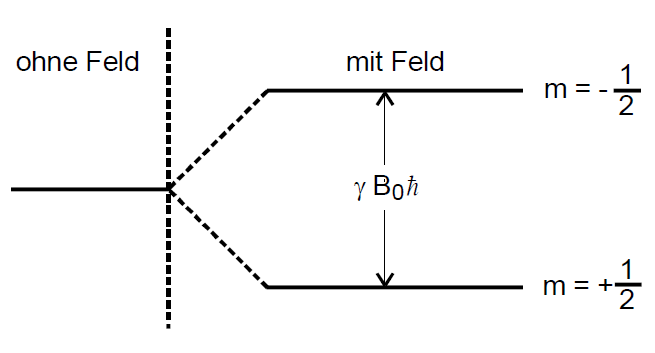
\includegraphics[width=8cm]{images/aufspaltung_magnetfeld.png}
\caption{Toller Titel (1)}
\label{fig_aufspaltung}
\end{figure}
Für die Exponentialfunktion in \ref{eq_izallgemein} kann eine lineare Näherung eingesetzt werden, falls
\begin{align}
m\gamma B_0 \hbar \ll k_\text{B}T 
\end{align}
ist, welches für Magnetfelder in der Größenordnung von 1 Tesla und Temperaturen nahe der Zimmertemperatur gegeben ist.\\
Es ergibt sich
\begin{align}
\left\langle I_Z \right\rangle_{\text{P}}= -\frac{\hbar^2}{4}\frac{\gamma B_0}{k_\text{B}T}\hspace*{0.5cm}\text{.} \label{eq_iznahrung}
\end{align}
Da die Kernspinpolarisation im direkten Zusammenhang mit den magnetischen Momenten $\vec{\mu}_I$ stehen, ist eine makroskopische Magnetisierung $\vec{M_0}$ der Probe messbar, die durch die Summe aller Einzelmomente pro Volumen
\begin{align}
\vec{M_0}=\sum\limits_{i}^{}\frac{\mu_0\vec{\mu}_i}{V}
\end{align}
gegeben ist.\\
Es ist
\begin{align}
\left\langle \vec{M_0}_z \right\rangle =N\gamma \mu_0 \left\langle I_Z \right\rangle_{\text{P}} :=\left\langle M_0 \right\rangle\hspace*{0.5cm}\text{.}
\end{align}
Wird nun \ref{eq_iznahrung} eingesetzt, so ergibt sich
\begin{align}
\left\langle M_0 \right\rangle = N\frac{\hbar^2}{4}\mu_0\frac{\gamma^2 B_0}{k_\text{B}T}:=M_0
\end{align}
als Gleichgewichtsmagnetisierung bei Temperatur $T$.
\subsection{Larmor-Präzession}
Damit das System interessantes Verhalten zeigt, muss $\vec{M}$ aus der Gleichgewichtslage $\vec{M_0}$ durch Hochfrequenzquanten mit Energie $\Delta E$ gebracht werden.\\
Außerdem kann das System klassisch betrachtet werden, da die Magnetisierung durch $N$ Spins mit $N \sim 10^{28}$ m$^{-2}$ erzeugt werden und folglich Quanteneffekte nicht relevant sind.\\
Es wirkt somit ein Drehmoment
\begin{align}
\vec{D}=\vec{M}\times B_0 \vec{e_z}
\end{align}
und es lässt sich dadurch über die Kreiselgleichung die Differenzialgleichung
\begin{align}
\frac{d \vec{M}}{d t} = \gamma \vec{M}\times B_0 \vec{e_z}\label{eq::magzeit}
\end{align}
herleiten.\\
Die komponentenweise Lösung der Differenzialgleichung ist durch
\begin{align}
M_x&= 0 \\
M_y&= A \cos \gamma B_0 t \\
M_z&= -A \sin \gamma B_0 t
\end{align}
gegeben.\\
Es folgt eine Präzession um $\vec{e_z}$-Achse mit der Larmor-Frequenz genannten Frequenz
\begin{align}
\omega_L =\gamma B_0 \hspace*{0.5cm}\text{.}
\end{align}
\subsection{Relaxationserscheinungen}
Der zeitliche Verlauf der Magnetisierung ist durch die Blochschen Gleichungen gegeben, die eine Zusammensetzung aus der Kreiselgleichung und der Differentialgleichung für die Relaxion besteht.\\
In diesen Fall lauten sie
\begin{align}
\frac{d M_x}{d t}&= \gamma B_0 M_y - \frac{M_x}{T_2}\label{eq::bloch1}\\
\frac{d M_y}{d t}&= \gamma B_0 M_x - \frac{M_y}{T_2}\label{eq::bloch2}\\
\frac{d M_z}{d t}&= \frac{M_0-M_Z}{T_1}\hspace*{0.5cm}\text{.}\label{eq::bloch3}
\end{align}
Es wurden dabei zwei Zeitkonstanten $T_1$ und $T_2$ eingeführt.\\
Die Zeitkonstante $T_1$ wird auch longitudinale oder Spin-Gitter-Relaxationszeit genannt, sie beschreibt die zeitliche Veränderung der Magnetisierungskomponente parallel zur Feldrichtung $\vec{B_0}$. Andererseits beschreibt sie auch den Energiefluss zwischen den Kernspinsystem und den Gitterschwingungen.\\
$T_2$ beschreibt hingegen die transversale Änderung. Sie wird auch Spin-Spin-Relaxationszeit, da die Abnahme der Magnetisierung senkrecht zur Feldrichtung $\vec{B_0}$ häufig durch Spin-Spin-Wechselwirkungen geschieht.
\subsection{HF-Einstrahlungsvorgänge}
Ein Hochfrequenzfeld mit Magnetfeld $\vec{B_1} \perp \vec{e_z}$ lässt sich durch
\begin{align}
\vec{B_{\text{HF}}}=2\vec{B_1} \cos \omega t
\end{align}
beschreiben.\\
Das Feld ist in zwei zirkular polarisierte Felder $\omega_+$ und $\omega_-$ aufteilbar.\\
Wenn $\omega_+$ nahe der Larmor-Frequenz $\omega_L$ ist, so ist der Beitrag von $\omega_-$ vernachlässigbar.\\
Es handelt sich dann um ein rotierendes Feld um die $\vec{e_x}$ und $\vec{e_y}$-Achse und es wirkt als gesamtes Magnetfeld auf die Probe
\begin{align*}
B_x=B_1 \cos \omega t \hspace*{0.1cm}\text{,}\hspace*{0.4cm} B_y=B_1 \sin \omega t \hspace*{0.3cm}\text{und}\hspace*{0.3cm} B_z=B_0\hspace*{0.1cm}\text{.}
\end{align*}
Es ist sinnvoll das Koordinatensystem in ein Koordinatensystem mit Zeitabhängigen Einheitsvektoren mit
\begin{align}
\frac{\partial \vec{\tilde{e_x}}}{\partial t}= -\vec{\omega} \times \vec{e_x}\hspace*{0.1cm}\text{,}\hspace*{0.4cm}
\frac{\partial \vec{\tilde{e_y}}}{\partial t}= -\vec{\omega} \times \vec{e_y}\hspace*{0.3cm}\text{und}\hspace*{0.3cm}
\frac{\partial \vec{\tilde{e_z}}}{\partial t}= 0
\end{align}
zu überführen.\\
Dadurch kann die Differenzialgleichung 
\begin{align}
\frac{d \vec{M}}{d t}= \gamma \vec{M}\times \left(\vec{B}_{\text{ges}}+\frac{\vec{\omega}}{\gamma}\right)
\end{align}
gewonnen werden, die die Form der Gleichung \ref{eq::magzeit} mit effektiven Magnetfeld
\begin{align}
\vec{B}_\text{eff}=\vec{B}_0+\vec{B}_1+\frac{\vec{\omega}}{\gamma}
\end{align}
hat.\\
Analog folgt auch eine Präzessionsbewegung, jedoch um die Feldrichtung von $\vec{B}_{\text{eff}}$.\\
Im Fall der Resonanz, also $\omega=\omega_L$ folgt, dass $\vec{B}_{\text{eff}}=\vec{B}_1$ ist und das magnetische Moment um die $\vec{B}_1$-Achse präzediert. Der Präzessionskegel ist dabei um $90^\circ$ geöffnet.\\
Der Drehwinkel $\delta\left(\delta t\right)$ ist durch
\begin{align}
\delta\left(\Delta t\right)=\gamma B_1 \Delta t
\end{align}
berechenbar.\\
Es lässt sich die Einstrahlzeit 
\begin{align}
\Delta t_{90}=\frac{\pi}{2\gamma B_1} 
\end{align}
bestimmen, die es benötigt bis $\vec{M}$ von der $-\vec{e_z}$ Richtung in die  $\vec{e_y}$ gedreht ist.\\
Analog kann $\Delta t_{180}=2 \Delta t_{90}$ bestimmt werden, bis $\vec{M}$ von der $\vec{e_z}$ Richtung in die  $-\vec{e_z}$ gedreht ist.\\ 
Durch das Relaxieren der Magnetisierung zurück in die Ruhelage können $T_1$ und $T_2$ bestimmt werden.
\subsection{Freier Induktionszerfall}
Ein Elektro- oder Permanentmagnet erzeugt ein homogenes Feld $B_0\vec{e_z}$. 
Senkrecht dazu ist eine Spule, in dessen Innenraum sich die Probe befindet. Der Aufbau ist in Abbildung \ref{fig::aufbau} abgebildet.
\begin{figure}[H]
\centering
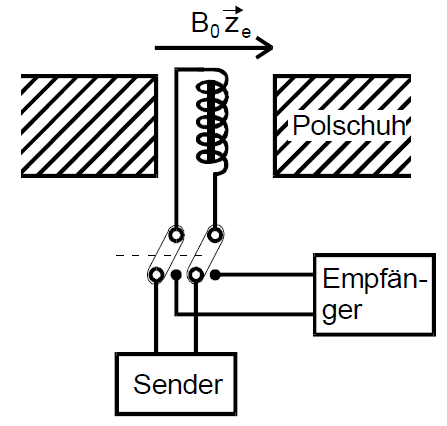
\includegraphics[width=8cm]{images/versuchsaufbau.png}
\caption{Toller Titel (1)}
\label{fig::aufbau}
\end{figure}
Durch die Spule wird ein hochfrequenter Strom geschickt, der ein hochfrequentes Magnetfeld erzeugt, welches die Anforderungen aus Kapitel 2.4 erfüllt, also ein in x-y Ebene umlaufendes Feld besitzt.\\
Es folgt ein $\Delta t_{90}$ Impuls, sodass die Magnetisierung in Richtung $\vec{e}_y$ liegt. Dadurch führt $\vec{M}$ eine Präzession auf der $\vec{e}_x$-$\vec{e}_y$-Ebene durch.\\
Das System erreicht durch Relaxationsprozesse mit der Zeit die Ausgangslage $\vec{M_0}$.\\
Dieser Prozess wird freier Induktionszerfall genannt.\\
Die Messung ist möglich, da durch die Präzession um $\vec{e}_x$-$\vec{e}_y$ eine Spannung in der Spule induziert wird, die vom Empfänger aufgenommen werden kann.\\
Nun ist das statische Feld $B_0$ nicht für alle Spins gleich stark. Dies hat sowohl physikalische als auch apparative Ursachen.\\
Zum einen sind die einzelnen Spins zusätzlichen Feldern, wie Dipolfeldern aus der nächsten Nachbarn-Wechselwirkung unterworfen, zum anderen kann durch die endliche Ausdehnung der Apparatur das Magnetfeld nicht völlig homogen sein.\\
Dadurch sind die Larmorfrequenzen lokal unterschiedlich, was zu unterschiedlichen Laufzeiten der Spins führt und somit zu einer Dephasierung.\\
Das gemessene $T_2^*$ unterscheidet sich vom realen $T_2$ durch
\begin{align}
\frac{1}{T_2^*}=\frac{1}{T_2}+\frac{1}{T_{\Delta B}}\hspace*{0.5cm}\text{.}
\end{align}
Die Störung $T_{\Delta B}$ durch das endliche Magnetfeld ist von der Größenordnung $\left(\gamma d G\right)^{-1}$ mit den Probendurchmesser $d$ und den Gradient $G$  des $\vec{B}_0$ Feldes.\\
Solange das B-Feld hinreichend homogen ist, also $T_{\Delta B} \ll T_2$ ist, ist eine Messung sinnvoll, da die Fehler dann meistens allein durch die Apparatur gegeben sind.
\subsection{Das Spin-Echo-Verfahren}
Die im vorigen Abschnitt genannten Störeffekte sind eliminierbar, wenn zeitlich konstant. Dafür werden zwei HF-Pulse verwendet.\\
Zunächst wird ein $90^\circ$-Puls gesendet, der die Magnetisierung entlang $\vec{\tilde{e}}_y$. Die Spins präzedieren während des Zeitraum $\tau \gg \Delta t_{90}$ um die $\vec{e}_z$ Achse.\\
Da die Spins mit der Zeit außer Phase geraten, bewegt sich ein Teil in Uhrzeigersinn, und der andere Teil entgegengesetzt.\\
Nach $\tau$ wird ein $180^\circ$-Puls gesendet, der die Spins flippt. Dadurch laufen die beiden Mengen an Spins wieder zusammen.
\begin{figure}[H]
\centering
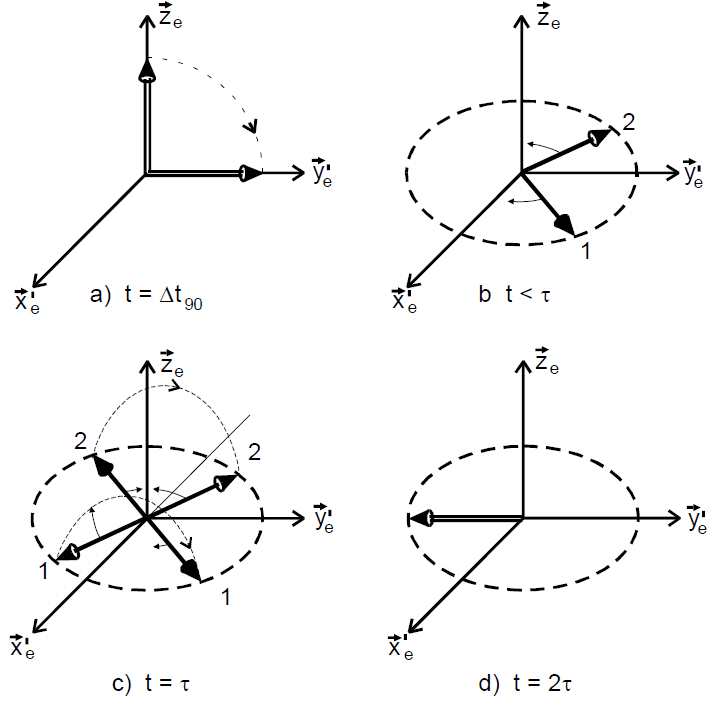
\includegraphics[width=12cm]{images/spin_echo.png}
\caption{Toller Titel (1)}
\label{fig::spin_echo}
\end{figure}
Es entstehen dabei nur Signale, wenn die beiden Teile nahe beieinander sind. Es entsteht ein Signal der Form \ref{fig::hahn_echo_verlauf}.\\
Diese Methode wird Hahn-Echo genannt.
\begin{figure}[H]
\centering
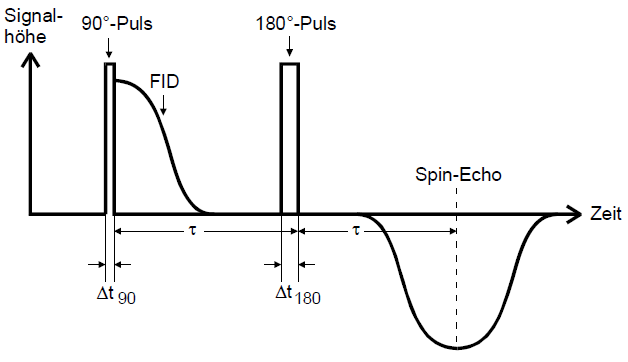
\includegraphics[width=12cm]{images/hahn_echo.png}
\caption{Toller Titel (1)}
\label{fig::hahn_echo_verlauf}
\end{figure}
\begin{figure}[H]
\centering
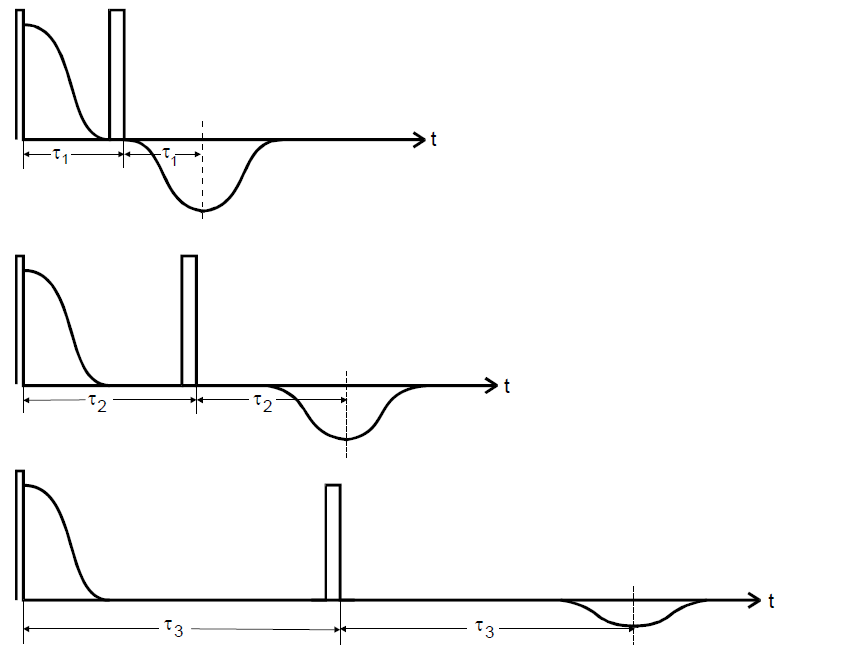
\includegraphics[width=12cm]{images/tauechohoehe.png}
\caption{Toller Titel (1)}
\label{fig::tauechohoehe}
\end{figure}
Im Grenzfall $T_2 \to \infty$ erreicht das Echosignal die ursprüngliche Höhe, jedoch besitzt das Signal ein umgekehrtes Vorzeichen.\\
Die Wechselwirkung der Spins mit ihrer Umgebung sorgt jedoch dafür, dass einige Spins nach $2\tau$ nicht in Phase sind und somit die Höhe des Signals abnimmt. Je größer die Zeit $\tau$ ist, desto stärker ist der Effekt, wie in Abbildung \ref{fig::tauechohoehe} zu sehen ist.\\
Der Zusammenhang ist durch
\begin{align}
M_y\left(t\right)=M_0\exp \left(-\frac{t}{T_2}\right)\label{eq::rechnung_tau_spin_echo}
\end{align} 
gegeben, dabei ist $M_y$ die Höhe des Spin-Echos.\\ 
Es lässt sich $T_2$ durch Variation von $\tau$ messen.
\subsection{Carr-Purcell- und Meiboom-Gill-Methode}
Da nach jeder Messung das System die ursprüngliche Gleichgewichtsmagnetisierung $M_0$ in z-Richtung zurück kehren muss, ist die im vorherigen Abschnitt beschriebene Spin-Echo-Methode zeitintensiv.\\
Eine Abhilfe schafft dabei die von Carr und Purcell vorgeschlagenen Methode, nach der zunächst analog wie bei der Spin-Echo-Methode ein $90^\circ$ Puls, jedoch wird anstatt einen $180^\circ$ Puls mehrere $180^\circ$ Pulse mit äquidistant Abstand $2\tau$ aufeinanderfolgen gesendet, wie in Abbildung \ref{fig::Carr_Purcellt_signal} dargestellt.
\begin{figure}[H]
\centering
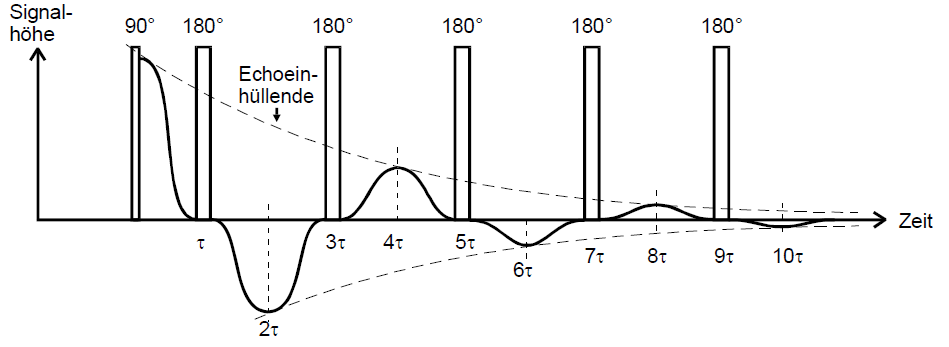
\includegraphics[width=14cm]{images/Carr_Purcellt_signal.png}
\caption{Toller Titel (1)}
\label{fig::Carr_Purcellt_signal}
\end{figure}
Da die Spins nach $2n\tau$ $n\in \mathbb{N}$ erneut fokussieren, befindet sich an diesen Stellen ein Extremum mit alternierendem Vorzeichnen.\\
Dabei nimmt die Echoamplitude mit der Zeit durch Relaxionsprozesse ab und es ist eine Messung nach \ref{eq::rechnung_tau_spin_echo} möglich.\\
Diese Methode liefert jedoch nur exakte Werte, wenn die $180^\circ$ Pulse exakt justiert sind. Ist dies nicht der Fall, so werden die Spins mit jedem Puls aus Messebene herausdreht.\\ Die Lösung ist, dass jeder zweite $180^\circ$ so justiert wird, dass die Spins wieder in der Messebene liegen. Dies wird als Meiboom-Gill-Methode bezeichnet.
\begin{figure}[H]
\centering
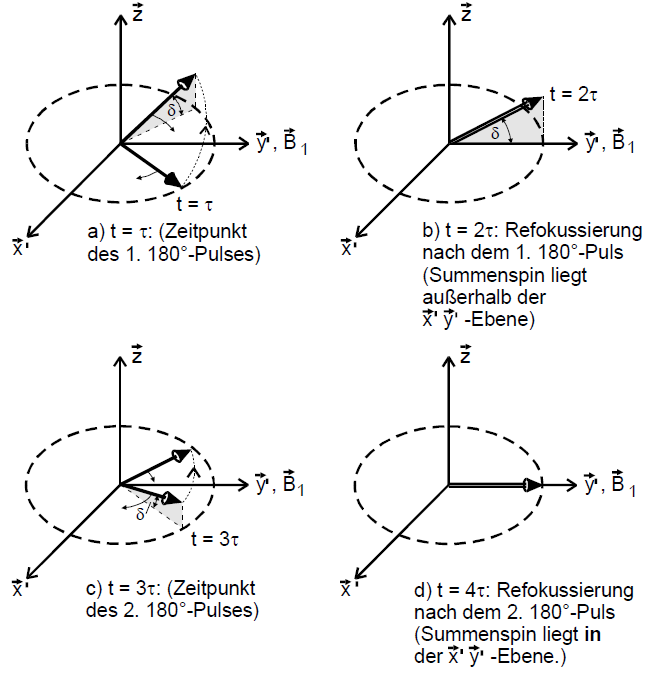
\includegraphics[width=14cm]{images/Meiboom_Gill_Methode.png}
\caption{Toller Titel (1)}
\label{fig::Meiboom_Gill_Methode}
\end{figure}
Wird nun jedes zweite Signal verwendet, so sind die Messergebnisse exakt.
\subsection{Einfluss der Diffusion}
Die Gleichung \ref{eq::rechnung_tau_spin_echo} ist nur für Statische Felder $B_0$ gültig.\\
Treten im Medium Erscheinungen wie die Brownscher Molekularbewegung auf, so bewegen sich die Spins in andere Teile des Systems mit anderem Magnetfeld. Die Lamorfrequenz wird deshalb zeitabhängig.\\
Dies führt zu einer schnelleren Abnahme des Signals als nach Gleichung \ref{eq::rechnung_tau_spin_echo} berechnet.\\
Es muss eine Diffusionskonstante $D$ eingeführt werden und die Blochschen Gleichungen \ref{eq::bloch1} - \ref{eq::bloch3} um
\begin{align}
\frac{\partial M}{\partial t} = D\Delta M \label{eq::bloch_diffusion}
\end{align} 
ergänzt werden.\\
Wird die Inhomogenität des Magnetfeldes $B_0$ und die Folge der Impulse berücksichtigt, so lässt sich die Funktion
\begin{align}
A\left(2n\tau\right)= \exp\left( - \frac{2}{3} D\gamma^2G^2\tau^3n\right)
\end{align}
für die Amplitude mit den Gradient $G$ des Magnetfeldes $B_0$ berechnen.\\
Die Magnetisierungsamplitude nimmt demnach exponentiell mit einer Zeitkonstanten
\begin{align}
T_D:=\frac{3}{D\gamma^2G^2\tau^2}
\end{align}  
ab. Diese Abnahme muss in \ref{eq::rechnung_tau_spin_echo} ergänzt werden, sodass sich
\begin{align}
M_y\left(t\right)=M_0\exp \left(-\frac{t}{T_2}\right)\exp \left(-\frac{t}{T_D}\right)
\end{align}
für die Amplitude ergibt.\\
Es fällt auf, dass eine Messung nach Carr-Purcell- oder Meiboom-Gill möglich ist, wenn $T_D$ groß gegen $T_2$ ist.\\
Andererseits kann die Diffusionskonstante durch Spin-Echo-Methode bestimmbar werden.
Dafür wird die Zeit $\tau$ zwischen den  $90^\circ$ und  $180^\circ$ Puls variiert und die Amplitude des 1. Echos gemessen. Es ergibt sich dann mit $t=2\tau$
\begin{align}
M_y\left(t\right)=M_0\exp \left(-\frac{t}{T_2}\right)\exp \left(-\frac{D\gamma^2G^2t^3}{12}\right)\hspace*{0.5cm}\text{.}
\end{align}
Dies gilt solange
\begin{align}
T_2^3 \gg \frac{12}{D\gamma^2 G^2}
\end{align}
gegeben ist.
\subsection{Spin-Gitter-Relaxationszeit T$_1$}
Für die Bestimmung von $T_1$ wird zunächst ein $180^\circ$ Puls gesendet, der die Probe aus ihrer Gleichgewichtslage auslenkt.\\
Nach der Zeit $\tau$ wird ein $90^\circ$ Puls geschickt, sodass ein Signal 
\begin{align}
M_{z}(\tau)=M_0(1-2\exp(-\tau/T_1))
\label{eq_T1}
\end{align}
gemessen werden kann.
\section{Durchführung}

\section{Auswertung}

\subsection{Bestimmung der Relaxationszeit T$_2$}
Unter der Annahme,dass die T$_D$ groß gegen T$_2$ ist, d.h. $\tau_1$ hinreichend klein ist, kann der Einfluss der Diffusion vernachlässigt werden. In diesem Fall ergibt sich für die Magnetisierung 
\begin{align}
M_Y(t)=M_0\exp\left( \frac{-t}{T_2}\right)\, ,
\end{align}
womit eine nicht-lineare Ausgleichsrechnung mit den Messwerten der Maxima aus der Meiboom-Gill-Methode durchgeführt werden kann.


\subsection{Berechnung des Diffusionskoeffizienten D}

\subsection{Bestimmung der Relaxationszeit T$_1$}
Die z-Komponente der Magnetisierung weist einen exponentiellen Zusammenhang mit dem Zeitabstand $\tau$ zwischen den 90$^{\circ}$ auf, wie in Formel \ref{eq_T1} dargestellt ist. \\
Zur Bestimmung von T$_1$ wird eine nicht-lineare Ausgleichsrechnung mit den in Tabelle \ref{tab_t1} angegebenen Messwerten durchgeführt. \\
\begin{center}
	\begin{tabular}{|c|c||c|c|}
		\hline	$\tau$ [s]	&	M$_z$ [V] & $\tau$ [s]	&	M$_z$ [V]\\
		\hline	0,003	&	1,47	&	1,503	&	-0,09	\\
		\hline	0,013	&	1,43	&	1,603	&	-0,12	\\
		\hline	0,023	&	1,41	&	1,703	&	-0,18	\\
		\hline	0,043	&	1,39	&	1,803	&	-0,24	\\
		\hline	0,063	&	1,37	&	1,903	&	-0,29	\\
		\hline	0,083	&	1,35	&	2,003	&	-0,3	\\
		\hline	0,103	&	1,31	&	2,203	&	-0,47	\\
		\hline	0,153	&	1,27	&	2,403	&	-0,58	\\
		\hline	0,203	&	1,21	&	2,603	&	-0,67	\\
		\hline	0,253	&	1,17	&	2,803	&	-0,75	\\
		\hline	0,303	&	1,13	&	3,003	&	-0,82	\\
		\hline	0,353	&	1,07	&	3,203	&	-0,9	\\
		\hline	0,403	&	1,01	&	3,403	&	-0,95	\\
		\hline	0,503	&	0,91	&	3,603	&	-1,01	\\
		\hline	0,603	&	0,81	&	3,803	&	-1,06	\\
		\hline	0,703	&	0,68	&	4,003	&	-1,1	\\
		\hline	0,803	&	0,58	&	4,503	&	-1,2	\\
		\hline	0,903	&	0,48	&	5,003	&	-1,28	\\
		\hline	1,003	&	0,38	&	5,503	&	-1,33	\\
		\hline	1,103	&	0,3	&	6,003	&	-1,34	\\
		\hline	1,203	&	0,2	&	7,003	&	-1,42	\\
		\hline	1,303	&	0,12	&	8,003	&	-1,44	\\
		\hline	1,403	&	0,04	&	9,003	&	-1,47	\\
		\hline
	\end{tabular}
	\captionof{table}{Aufgenommene Messwerte der z-Komponente der Magnetisierung in Abhängigkeit vom Zeitabstand $\tau$ zwischen den 90$^{\circ}$-Pulsen.}
	\label{tab_t1}
\end{center}
Mit Gleichung \ref{eq_T1} ergibt eine nicht-lineare Ausgleichsrechnung mit Python folgende Fitparameter:
\begin{align*}
M_0&=(1.51 \pm 0.01)\si{V} \\
T_1&=(2.08 \pm 0.01)\si{s}
\end{align*}

\subsection{Bestimmung der Viskosität $\eta$}

\subsection{Berechnung des Molekülradius r von Wasser}
\section{Quellen}

\end{document}